\section{Introduction}
\label{sec:intro}

Modern video diffusion models~\citep{ho2022video, blattmann2023stable, wang2025wan} have driven a 
growing line of controllable interactive world models
~\citep{bruce2024genie, parkerholder2024genie2, parkerholder2025genie3, alonso2024diffusion, feng2024matrix, 
zhang2025matrixgame, he2025matrixgame2, valevski2024diffusion, oasis2024} to near-cinematic fidelity,
yet every such system inherits a structural limitation from the rendering pipelines it replaces:
actions are bound to engine-internal animation namespaces or device-level inputs, 
locking action semantics to a specific entity and engine.
This entity-and-engine binding forces a separate action vocabulary to be designed 
for every entity in every world,
making cross-entity and cross-world generalization an engineering burden rather 
than a modeling choice.
We argue that this is not an intrinsic property of multi-entity interactive video,
but a property of the \emph{action interface}: the protocol through which a user specifies what should
happen on the next frame, and replacing it fundamentally expands what such a model can express.
% Modern video diffusion models~\citep{ho2022video, blattmann2023stable, wang2025wan} now drive a growing line of controllable interactive world models~\citep{bruce2024genie, parkerholder2024genie2, parkerholder2025genie3, alonso2024diffusion, feng2024matrix, zhang2025matrixgame, he2025matrixgame2, valevski2024diffusion, oasis2024} to near-cinematic fidelity under a single shared camera, yet every such system inherits a structural limitation from the rendering pipelines it replaces: actions are bound either to engine-internal animation namespaces or to device-level inputs, both of which lock action semantics to a specific entity, body, and engine.
% Margit's animation~\#50, the Crucible Knight's animation~\#50, and animation~\#50 in any other engine refer to entirely unrelated events; the same is true of every keyboard mapping.
% As a consequence, an action defined for one entity cannot be issued to another, even when both share the scene, the camera, and the underlying motor primitives. We argue that this is not a property of multi-entity video as a problem, but a property of the \emph{action interface}: the protocol through which a user specifies what should happen on the next frame, and replacing it changes what such a model can express.

This bottleneck dominates in the \emph{single-viewpoint multi-entity} regime: 
a shared camera with two or more independently controllable entities, 
as in RPG (Role-Playing Game) combat and PvP (Player vs. Player) fighting.
This regime is central to competitive and adversarial gameplay, yet remains 
structurally underserved by interactive video world models.
Most controllable interactive world models confine control to a single entity,
leaving the rest as passive scenery~\citep{bruce2024genie, oasis2024, he2025matrixgame2, 
guo2025mineworld}, 
while recent 
multi-entity attempts sidestep the regime by dropping joint dynamics~\citep{po2026multigen}, 
abandoning the shared camera~\citep{solaris2025}, 
or controlling only one side~\citep{agarwal2026combat}.
None of these approaches admits a protocol with both fine-grained multi-entity control
and generalization across entities and worlds.
This shortfall ultimately traces back to the \emph{action interface} itself, 
which exhibits two conventional failure modes: 
\textbf{($\mathbf{1}$) Engine-internal animation labels} 
(per-world discrete IDs~\citep{alonso2024diffusion} and per-entity namespaces) 
bind each index to a specific animation at design time, 
so rendering any out-of-vocabulary (OOV) action is inherently inexpressible.
\textbf{($\mathbf{2}$) Human-device inputs}~\citep{bruce2024genie, parkerholder2024genie2,parkerholder2025genie3, oasis2024, he2025matrixgame2, guo2025mineworld,yu2025gamefactory, valevski2024diffusion} and 
\textbf{scene-level captions}~\citep{che2024gamegenx, tang2025hunyuan, team2026advancing} 
operate at the granularity of the player or the holistic scene rather than the individual entity,
thus lacking the critical per-entity addressability (e.g.,~non-player characters).
A viable multi-entity interface must therefore deliver both \emph{open-vocabulary semantics} 
for cross-entity semantic sharing and \emph{per-entity addressability} 
for independent, simultaneous control of each entity.
% The bottleneck dominates in the \emph{single-viewpoint multi-entity} regime: a shared camera with two or more independently controllable entities, as in RPG combat and PvP fighting.
% This regime is central to competitive and adversarial gameplay, yet has been left structurally underserved by interactive video world models.
% Most controllable interactive world models confine control to a single entity, leaving the rest as passive scenery~\citep{bruce2024genie, oasis2024, he2025matrixgame2, guo2025mineworld}, and recent attempts to extend the setting do not address its full requirements: they either train a separate model per entity without joint dynamics~\citep{po2026multigen}, relax the single-camera constraint by giving each entity its own viewpoint~\citep{solaris2025}, or expose only one entity to control while generating the other reactively~\citep{agarwal2026combat}.
% None of these regimes admits a direct numerical comparison with the system we study: the protocols they evaluate (per-entity rollout, per-viewpoint rollout, single-side control) cannot host the per-frame per-entity action prompts that define our problem.
% The two conventional action interfaces fail this regime in distinct ways.
% \textbf{(1) Engine-internal animation labels} (per-world discrete IDs~\citep{alonso2024diffusion} and per-entity namespaces) bind each index at design time to a specific animation, so any action outside an entity's predefined inventory is, by construction, inexpressible.
% \textbf{(2) Human-device inputs}~\citep{bruce2024genie, parkerholder2024genie2, parkerholder2025genie3, oasis2024, he2025matrixgame2, guo2025mineworld, valevski2024diffusion} and scene-level captions~\citep{yu2025gamefactory, tang2025hunyuan, team2026advancing} operate at the granularity of the player or the scene rather than the individual entity.
% A viable multi-entity interface therefore needs both \emph{open-vocabulary semantics}, so meaning is shared across entities and worlds, and \emph{per-entity addressability}, so each entity is steerable through an independent simultaneous channel.

To address this limitation,
we propose \emph{a per-entity natural-language action interface} as the 
first to 
satisfy both desiderata, and present \methodname, 
the first interactive video world model 
supporting 
independent and simultaneous multi-entity control 
under a single shared viewpoint via 
per-frame natural-language conditioning
(\textbf{Throughout this paper, ``frame'' denotes a VAE-compressed latent frame 
unless otherwise specified; $\mathbf{1}$\,latent frame corresponds to $\mathbf{4}$\,pixel 
frames along the temporal axis; FPS denotes end-to-end pixel-frame throughput}).
Our interface assigns each entity its own 
syntactically isolated text segment within 
a shared prompt template at $0.25$\,s temporal 
granularity, enabling concurrent yet 
independent control of all entities.
Natural language shares semantics across entities by construction,
inherently allowing any action to be transferred from its 
native entity to another via a single textual phrase (Figure~\ref{fig:demo}).
We term this \emph{concept-level} cross-entity transfer: the model must 
synthesize both 
the motion and the visual concept on an entity that has no recording of the 
action, a capability inherently inaccessible to 
rendering pipelines bound to per-entity animation namespaces.
To our knowledge, no prior interactive video world model has explicitly addressed 
cross-entity action transfer at the level of per-frame, 
per-entity conditioning.
% We propose \emph{a per-entity natural-language action interface} as the first interface to satisfy both, and present \methodname, the first interactive video world model that supports independent and simultaneous multi-entity control under a single shared viewpoint via per-frame natural-language conditioning.
% Our interface assigns each entity its own dedicated, syntactically isolated text segment in a shared prompt template at $0.25$\,s temporal granularity, enabling concurrent yet independent control of all entities.
% Natural language shares semantics across entities by construction: the phrase \texttt{Tail of the Crucible} carries the same meaning whether issued to the Crucible Knight (its native owner) or to Margit, and the same alignment lets us render Margit executing the Knight's signature tail attack and the Knight wielding Margit's exclusive light blades (Figure~\ref{fig:demo}).
% This is \emph{concept-level} cross-entity transfer: from a textual phrase alone, the model must synthesize both the motion and the visual concept (a tail, a light blade) on a body that has no recording of the action. Rendering pipelines bound to per-entity animation namespaces cannot express such a transfer, since the concept itself lies outside the recipient's design-time inventory.
% To our knowledge, no prior interactive video world model has explicitly addressed cross-entity action transfer at the level of per-frame, per-entity conditioning; the same structural barrier underpins cross-embodiment action transfer in robotics, and we view our multi-entity setting as a concrete testbed for studying it through a language interface.

\begin{figure*}[t]
    \centering
    \captionsetup{justification=raggedright, singlelinecheck=false}
    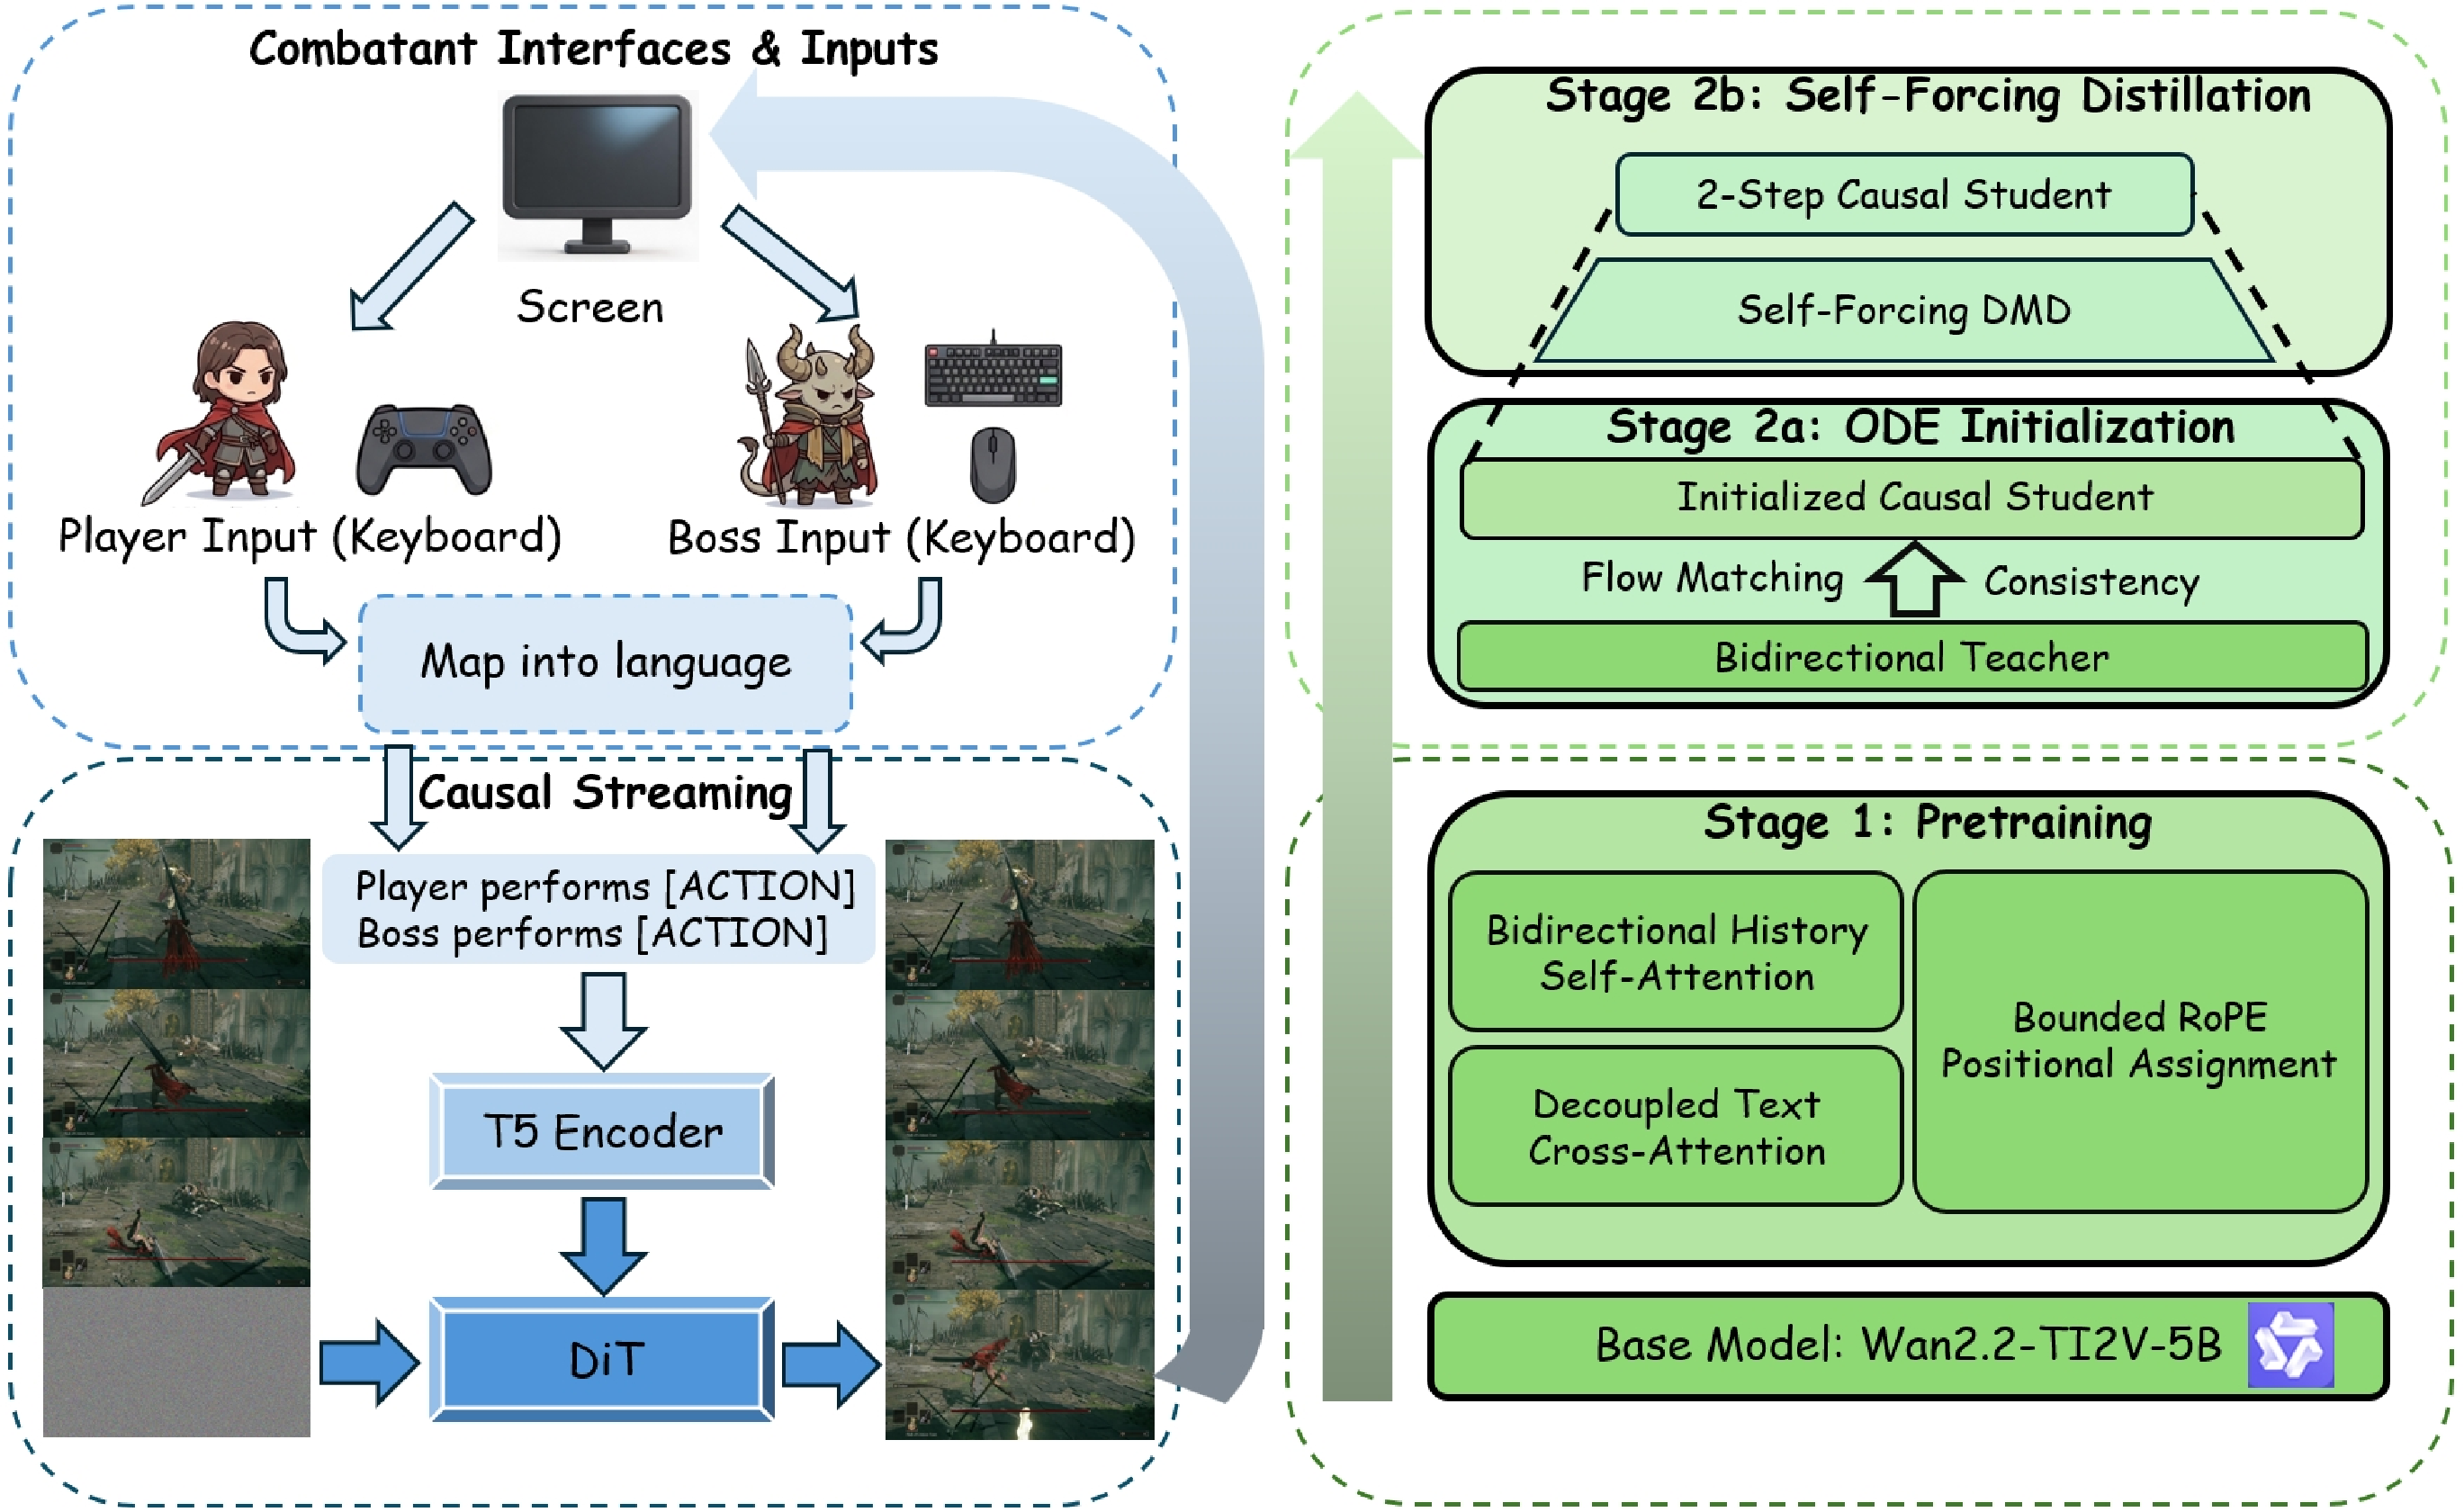
\includegraphics[width=\linewidth]{figures/fig_workflow.pdf}
    \caption{\textbf{Workflow of \methodname.}
    \textbf{Left:} \methodname translates combatant keyboard inputs into natural language prompts and autoregressively generates video frames in a causal streaming manner.
    \textbf{Right:} Training proceeds in two stages: ($1$)~Language-Conditioned Pretraining adapts the base model for per-frame text-driven generation; ($2$)~ODE-Initialized Self-Forcing Distillation enables real-time streaming via ODE-based flow matching initialization followed by Self-Forcing distillation.}
    \label{fig:workflow}
\end{figure*}

\methodname{} realizes this interface on top of a pretrained bidirectional video diffusion backbone~\citep{wang2025wan}. The core design is a \textbf{per-frame language-conditioned attention scheme}: decoupled text cross-attention is restricted exclusively to the noisy target frame and applied on top of bidirectional history self-attention, so each frame is steered by exactly its own action prompt without disturbing the backbone's pretrained priors or contaminating the committed history. We further enable real-time streaming inference by coupling ODE-initialized Self-Forcing distillation~\citep{chen2025selfforcing} with a RoPE-decoupled KV-cache sliding window, which collapses inference to two steps and keeps memory and positional geometry bounded over indefinite horizons.

Extensive experiments have demonstrated the structural advantage of \methodname{}'s 
natural-language interface. On cross-entity prompts (actions issued to entities 
that never executed them in training), \methodname{} attains $89\%$ Action 
Control Accuracy (ACA), far exceeding the $43\%$ of an Action-Index baseline 
whose accuracy merely tracks visual similarity rather than the action label 
itself. The gap widens to $90\%$ versus $0\%$ on OOV prompts, 
since the Action-Index interface cannot accept any prompt outside its fixed vocabulary. 
Besides its fine-grained per-frame control, \methodname{} sustains real-time long-horizon generation 
at $19.7$\,FPS with stable visual quality over $\mathbf{2}$-hour sessions, and replicates 
the performance on the visually unrelated \textit{King of Fighters} (KOF) world merely by 
vocabulary substitution alone, further validating its cross-world generalization capability. Our contribution can be summarized as follows:

\begin{enumerate}[leftmargin=*,topsep=1pt,itemsep=0pt]
\item We propose \textbf{natural language as the action interface for multi-entity video world models}, the first per-entity parallel control regime with open-vocabulary semantics, and demonstrate two structural capabilities unavailable to any discrete action-index, device-input, or scene-caption interface by construction: \textit{cross-entity action transfer} and \textit{out-of-vocabulary coverage}.
\item We present \methodname, the first interactive video world model with \textbf{per-frame, per-entity language conditioning} under a single shared viewpoint, achieving real-time multi-entity control for $\mathbf{>2}$ hours and reproducing its behavior on a second visually unrelated world under the same training recipe with vocabulary substitution as the only domain-specific change.
\item We construct a $128$-hour gaming dataset spanning two heterogeneous worlds (\textit{Elden Ring} and \textit{The King of Fighters}), the first dataset with \textbf{accurate per-frame, per-entity action labels} at $0.25$\,s temporal granularity, directly extracted from game memory at zero temporal offset.
\end{enumerate}

% Three controlled experimental axes show that the interface gain is structural rather than incremental.
% With architecture, data, and compute held identical, \methodname{} reaches $89\%$ Action Control Accuracy (ACA) on cross-entity prompts (actions issued to entities that never executed them in training), against $43\%$ for a hash-projected discrete-ID baseline and a ${\sim}6\%$ uniform-random baseline; the ID baseline's accuracy tracks visual similarity to the target entity's native moves rather than the shared action label, exposing it as a nearest-neighbour fallback rather than genuine semantic transfer.
% On out-of-vocabulary prompts the gap is structural by construction ($90\%$ vs.\ $0\%$), since the ID interface cannot accept any prompt outside its fixed vocabulary.
% These gaps reflect structural properties of the interface, not artifacts of evaluation size: our cross-entity protocol spans the full range of visual overlap between the two entities, and any discrete-ID baseline strengthened by aligning IDs to text-encoder features either reduces to natural-language conditioning at inference or, if it discards the text encoder, remains unable to accept any out-of-vocabulary prompt by construction (\Cref{sec:robustness}, \Cref{app:stronger_id}).
% The $2$-step student sustains $0.16$\,s per frame at $480$p on a single H100, with FVD remaining within a tight band over continuous $\mathbf{2}$-hour sessions, matching the longest validated horizons reported by prior interactive video world models despite a training context of only $1.75$\,s.
% The same architecture replicates these results on the visually unrelated \textit{King of Fighters} world by vocabulary substitution alone, with no architectural modification.

% \paragraph{Contributions.}
% \begin{enumerate}[leftmargin=*,topsep=1pt,itemsep=0pt]
% \item We propose \textbf{natural language as the action interface for multi-entity video world models}, the first per-entity parallel control regime with open-vocabulary semantics, and show that it expresses two structural capabilities, cross-entity action transfer and out-of-vocabulary control, that no discrete-ID, keyboard, or scene-caption interface can express by construction.
% \item We present \methodname, the first interactive video world model with \textbf{per-frame, per-entity language conditioning} under a single shared viewpoint, achieving real-time multi-entity control over horizons exceeding $\mathbf{2}$ hours and reproducing its behavior on a second visually unrelated world by vocabulary substitution alone.
% \item We construct a $128$-hour gaming dataset spanning two heterogeneous worlds (\textit{Elden Ring} and \textit{The King of Fighters}), the first dataset with \textbf{accurate per-frame, per-entity action labels} at $0.25$\,s temporal granularity, directly extracted from game memory at zero temporal offset.
% \end{enumerate}

% =====================================================================
% Previous oral-style draft (kept for reference / quick rollback).
% =====================================================================
% A central structural limitation of every interactive video world
% model to date is the boundary it inherits from the rendering pipelines
% it replaces: actions are bound either to engine-internal animation
% namespaces or to device-level inputs, both of which lock action
% semantics to a specific entity, body, and engine. ...
% Replacing this interface with \emph{per-frame, per-entity natural
% language} removes the boundary by construction. ...
% [full previous draft omitted for brevity; see git history]

% =====================================================================
% Original active version before any rewrite (kept for reference).
% =====================================================================
% Video diffusion models~\citep{ho2022video, blattmann2023stable, wang2025wan} have achieved
% remarkable success in
% generating near-cinematic video, and a growing line of works
% have extended them into controllable interactive
% world models~\citep{bruce2024genie, parkerholder2024genie2, parkerholder2025genie3,
% alonso2024diffusion, feng2024matrix, zhang2025matrixgame, he2025matrixgame2, valevski2024diffusion,
% oasis2024}.
% Most interactive videos operate under a single shared-camera viewpoint, encompassing first-person, third-person, and side-scrolling perspectives, each of which renders the entire scene within a single frame. Within this setting, existing world models have already delivered impressive visual fidelity.
% However, most of them are confined to the \emph{single-agent}
% control regime: only one entity (typically the player) is steered while all surrounding
% content remains passive scenery~\citep{bruce2024genie, oasis2024, he2025matrixgame2, guo2025mineworld}.
% This limitation hinders their extension to the modeling of adversarial \emph{multi-entity} scenarios,
% such as combatants in Role-Playing Games (RPGs) and Player-versus-Player (PvP) games,
% where every entity should mutually interact with others.
%
% Extending world models to this setting is non-trivial:
% \emph{single-viewpoint}, \emph{multi-entity} control must simultaneously preserve
% holistic scene coverage within one shared frame and expose every entity to independent
% interactive control.
% Though recent works have ventured into multi-entity control,
% none of them fully resolves both requirements:
% they either train a separate model per entity without simultaneous
% joint modeling~\citep{po2026multigen},
% relax the single-camera constraint by assigning
% each entity its own viewpoint rather than rendering the scene holistically~\citep{solaris2025} ,
% or expose only one of the two entities to direct control while generating the other reactively~\citep{agarwal2026combat}.
% To our best knowledge, no prior world model retains the
% standard single shared viewpoint
%  while granting independent and simultaneous controllability to every entity.
%
% We attribute the poor exploration of single-viewpoint multi-entity
% control to the discrete and separate \textbf{action interface}, the protocol through which
% a user specifies what should happen on the next frame and determines
% the action space a model can express.
% Conventional interfaces comprise two main control regimes:
% \textbf{(1) Engine-internal animation labels.}
% These include per-world discrete action identifiers (IDs)~\citep{alonso2024diffusion}
% and per-entity namespaces, where each index is bound to a
% specific animation at design time.
% Since actions sharing the same ID number across different entities are entirely unrelated events,
% such ID-based representations carry no shared semantics across entities or worlds,
% fundamentally limiting the expressiveness of multi-entity control.
% \textbf{(2) Human-device inputs.}
% These include input devices (e.g., keyboard, mouse, touchscreen)
% ~\citep{bruce2024genie, parkerholder2024genie2, parkerholder2025genie3,
% oasis2024, he2025matrixgame2, guo2025mineworld, valevski2024diffusion} and
% scene-level captions~\citep{yu2025gamefactory, tang2025hunyuan, team2026advancing},
% which operates at the granularity of the player or the scene rather than
% individual entities.
% This mismatch is critical: player operation signals cannot represent non-player entity actions,
% and a single scene-level caption cannot accurately address multiple simultaneously
% controllable entities.
% Motivated by these limitations, we identify two key properties that a viable multi-entity interface
% should satisfy:
% \textbf{(1) Open-vocabulary semantics.} The action representation is shared across entities and worlds;
% \textbf{(2) Per-entity addressability.} Each entity is steerable through independent, simultaneous control
% channels.
% We therefore propose \emph{natural language with parallel per-entity slots} as a novel multi-entity control
% interface:
% linguistic meaning naturally provides open-vocabulary semantics,
% while the parallel structure enables per-entity addressability.
%
% In this work, we present \methodname, the first interactive video world model that supports
% independent and simultaneous multi-entity control within a single shared viewpoint via
% per-frame natural language conditioning.
% Concretely, for each frame, our action interface represents each entity's control signal
% in a dedicated, syntactically isolated slot within a shared prompt template,
% enabling independent yet concurrent control over all entities.
% To accommodate this multi-entity control regime and support real-time long-horizon interaction,
% we adopt two architectural patterns:
% \textbf{(1) Per-Frame Language-Conditioned Backbone.}
% We introduce decoupled text cross-attention to ensure the exclusive control of per-frame language prompts, built upon a bidirectional history self-attention paradigm that
% preserves the pretrained priors of the bidirectional video diffusion backbone~\citep{wang2025wan}
% for stable and efficient training.
% \textbf{(2) Self-Forcing Distillation with Bounded Sliding Window.}
% We achieve two-step real-time streaming inference via
% ODE-initialized Self-Forcing distillation~\citep{chen2025selfforcing} paired with a
% RoPE-decoupled KV-cache sliding window, together enabling instant frame generation
% with bounded inference
% compute and constant positional geometry over long horizons.
%
% Extensive experiments demonstrate \methodname's exceptional
% interactive generation and fine-grained multi-entity control.
% \methodname achieves highly accurate action control (95\%) at 0.16s per frame,
% surpassing the traditional discrete-ID interface (89\%) under standard in-distribution conditions.
% The advantage widens substantially in cross-entity scenarios,
% where control prompts lie entirely outside the default entity vocabulary:
% \methodname maintains precise control (89\%) while discrete-ID degrades sharply
% on cross-entity inputs (43\%), evidencing the strong cross-entity semantic transfer
% enabled by our natural language interface.
% Furthermore, \methodname generalizes seamlessly to visually unrelated worlds without architectural modification,
% highlighting its unified applicability across diverse multi-entity world modeling settings.
% To summarize, our core contributions are:
% \begin{enumerate}[leftmargin=*,topsep=1pt,itemsep=0pt]
% \item We propose \textbf{natural language as the action interface} ---
% the first semantically general, per-entity parallel control regime for single-viewpoint multi-entity world modeling,
% with inherent robustness to cross-entity and cross-world generalization.
% \item We present \methodname, the first interactive world model with
% \textbf{per-frame language conditioning}, achieving real-time accurate multi-entity action control over
% horizons exceeding 2 hours.
% \item We construct a 128-hour gaming dataset spanning two heterogeneous worlds
% \textit{Elden Ring} and \textit{The King of Fighters} --- the first dataset with \textbf{accurate per-frame per-entity action labels}
% at a temporal granularity of 0.25s,
% which are automatically extracted from game memory at zero manual-annotation cost.
% \end{enumerate}
